
\section{Introduction}
\label{sec:intro}

Rapid growth in high-dimensional data from automated data sources~\cite{plato,macrobase-cidr} poses a scalability challenge for machine learning (ML) pipelines.
Dimensionality reduction (DR) techniques can alleviate this scalability challenge~\cite{keogh-indexing,local-dr,decade,gemini}.
In exchange for a runtime cost ($R$), DR methods transform an $n$-dimensional dataset to a lower $k$-dimensional representation while preserving salient dataset features, allowing downstream analytics routines to run in time proportional to $k$, while preserving downstream task accuracy .

Principal Component Analysis (PCA) is often practioners' DR method of choice with respect to transformation quality ($k$) for a target accuracy~\cite{jolbook}. 
However, na\"{i}ve, task-independent PCA implementations scale poorly, resulting in runtimes ($R$) that outweigh the downstream runtime benefit of DR. 
Thus, practitioners may sacrifice quality for end-to-end runtime, and use PCA alternatives~\cite{keogh-study}. 

Sample-based stochastic PCA algorithms~\cite{shamir,re-new} are a scalable alternative to classical PCA.
However, the amount of sampling required is data-dependent.
If we sample too many data points, PCA's runtime overhead would still outweigh its transformation quality.
If we sample too few data points, PCA may fail to deliver a sufficiently high-quality reduction and compromise the runtime and/or accuracy of downstream tasks.
Thus, we ask: can we develop a workload-dependent way to efficiently and accurately determine the sampling rate for stochastic PCA, so we can obtain PCA's transformation quality \emph{and} minimize workload runtime?

\begin{figure}
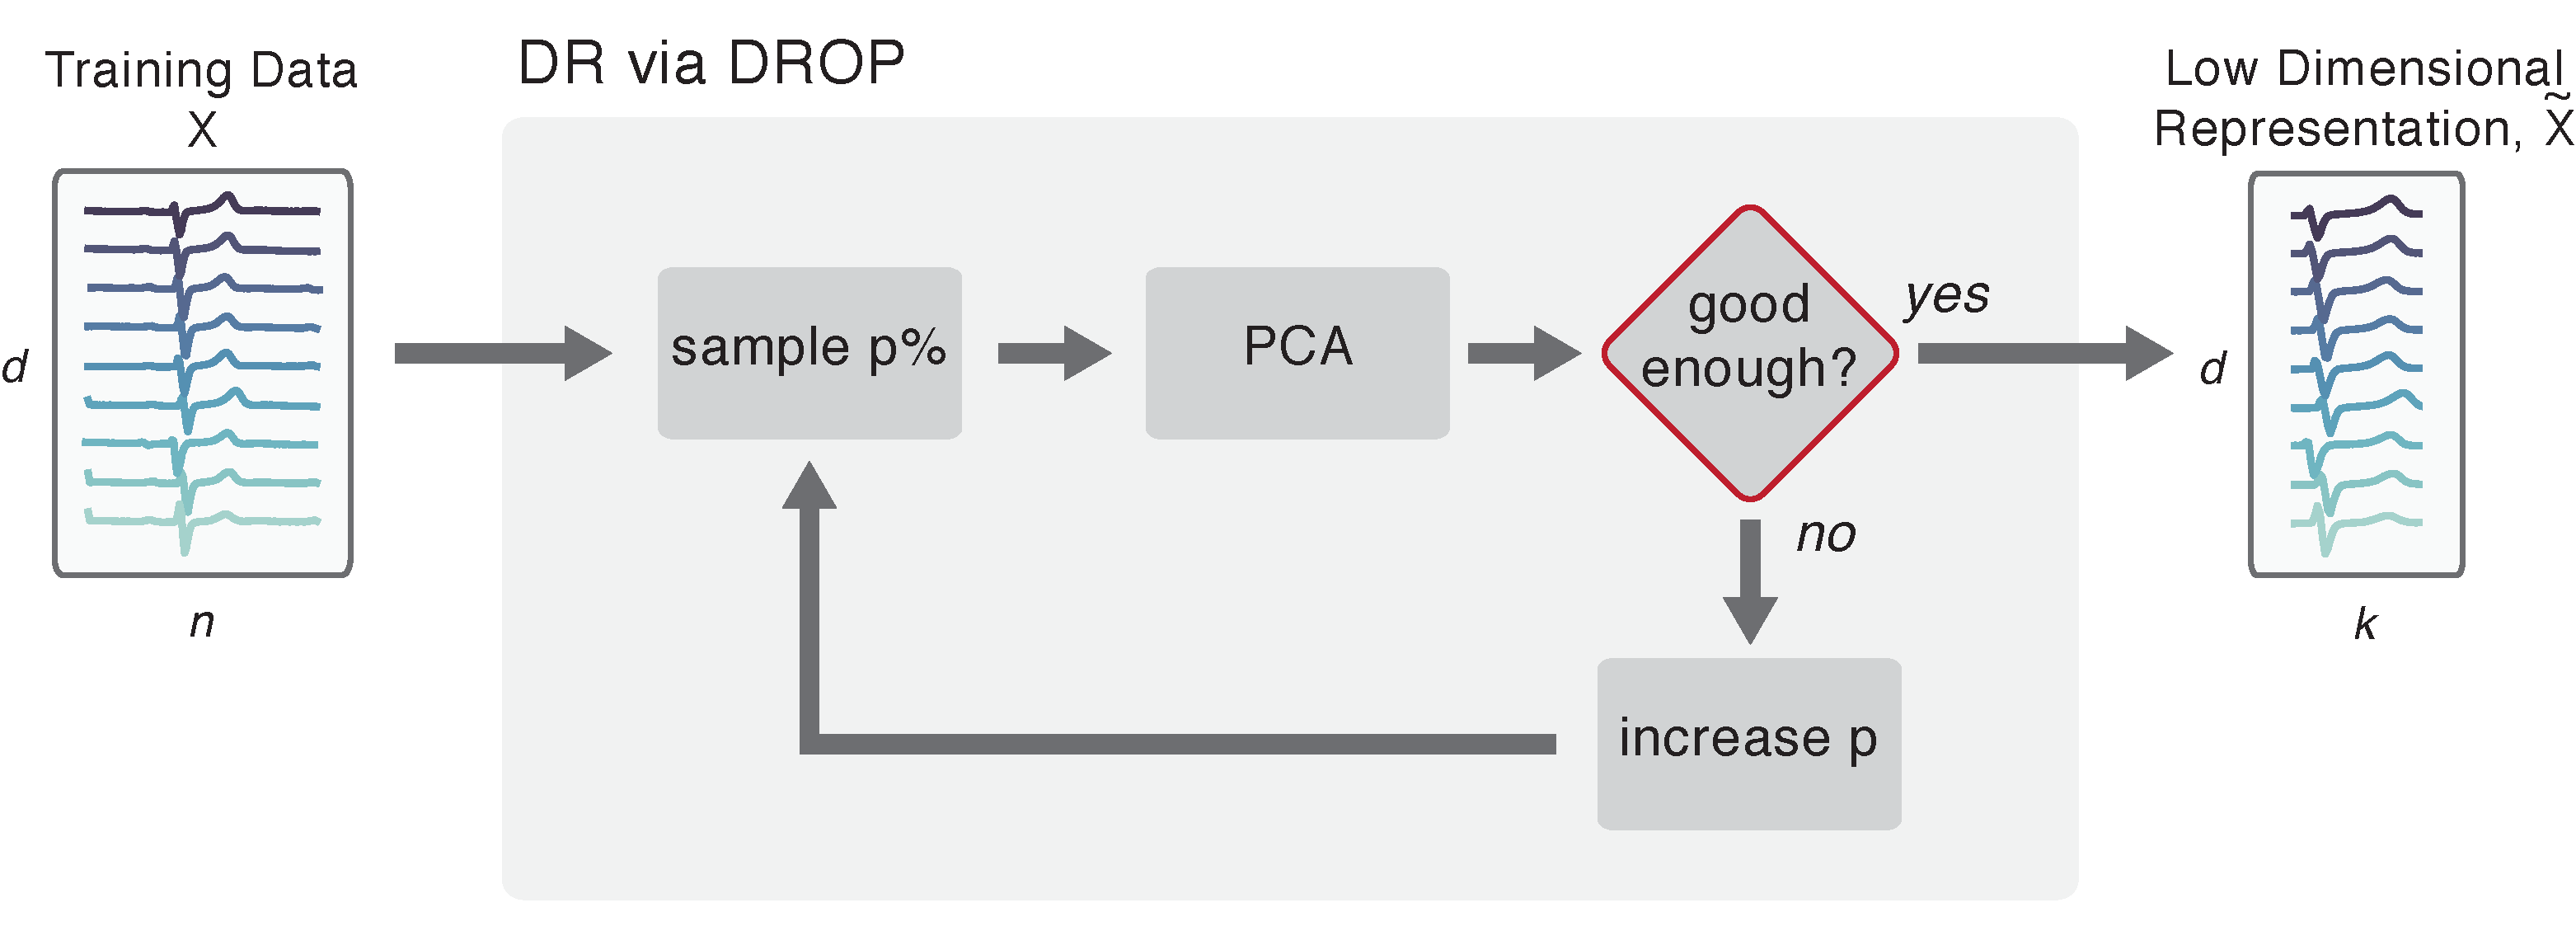
\includegraphics[width=\linewidth]{figs/basic.pdf}
\caption[]{DROP is a workload-aware DR operator compatible with standard ML pipelines. DROP solves the challenge of when to stop sampling (``good enough?")}
\label{fig:basic}
\end{figure}

\begin{comment}
\begin{figure}
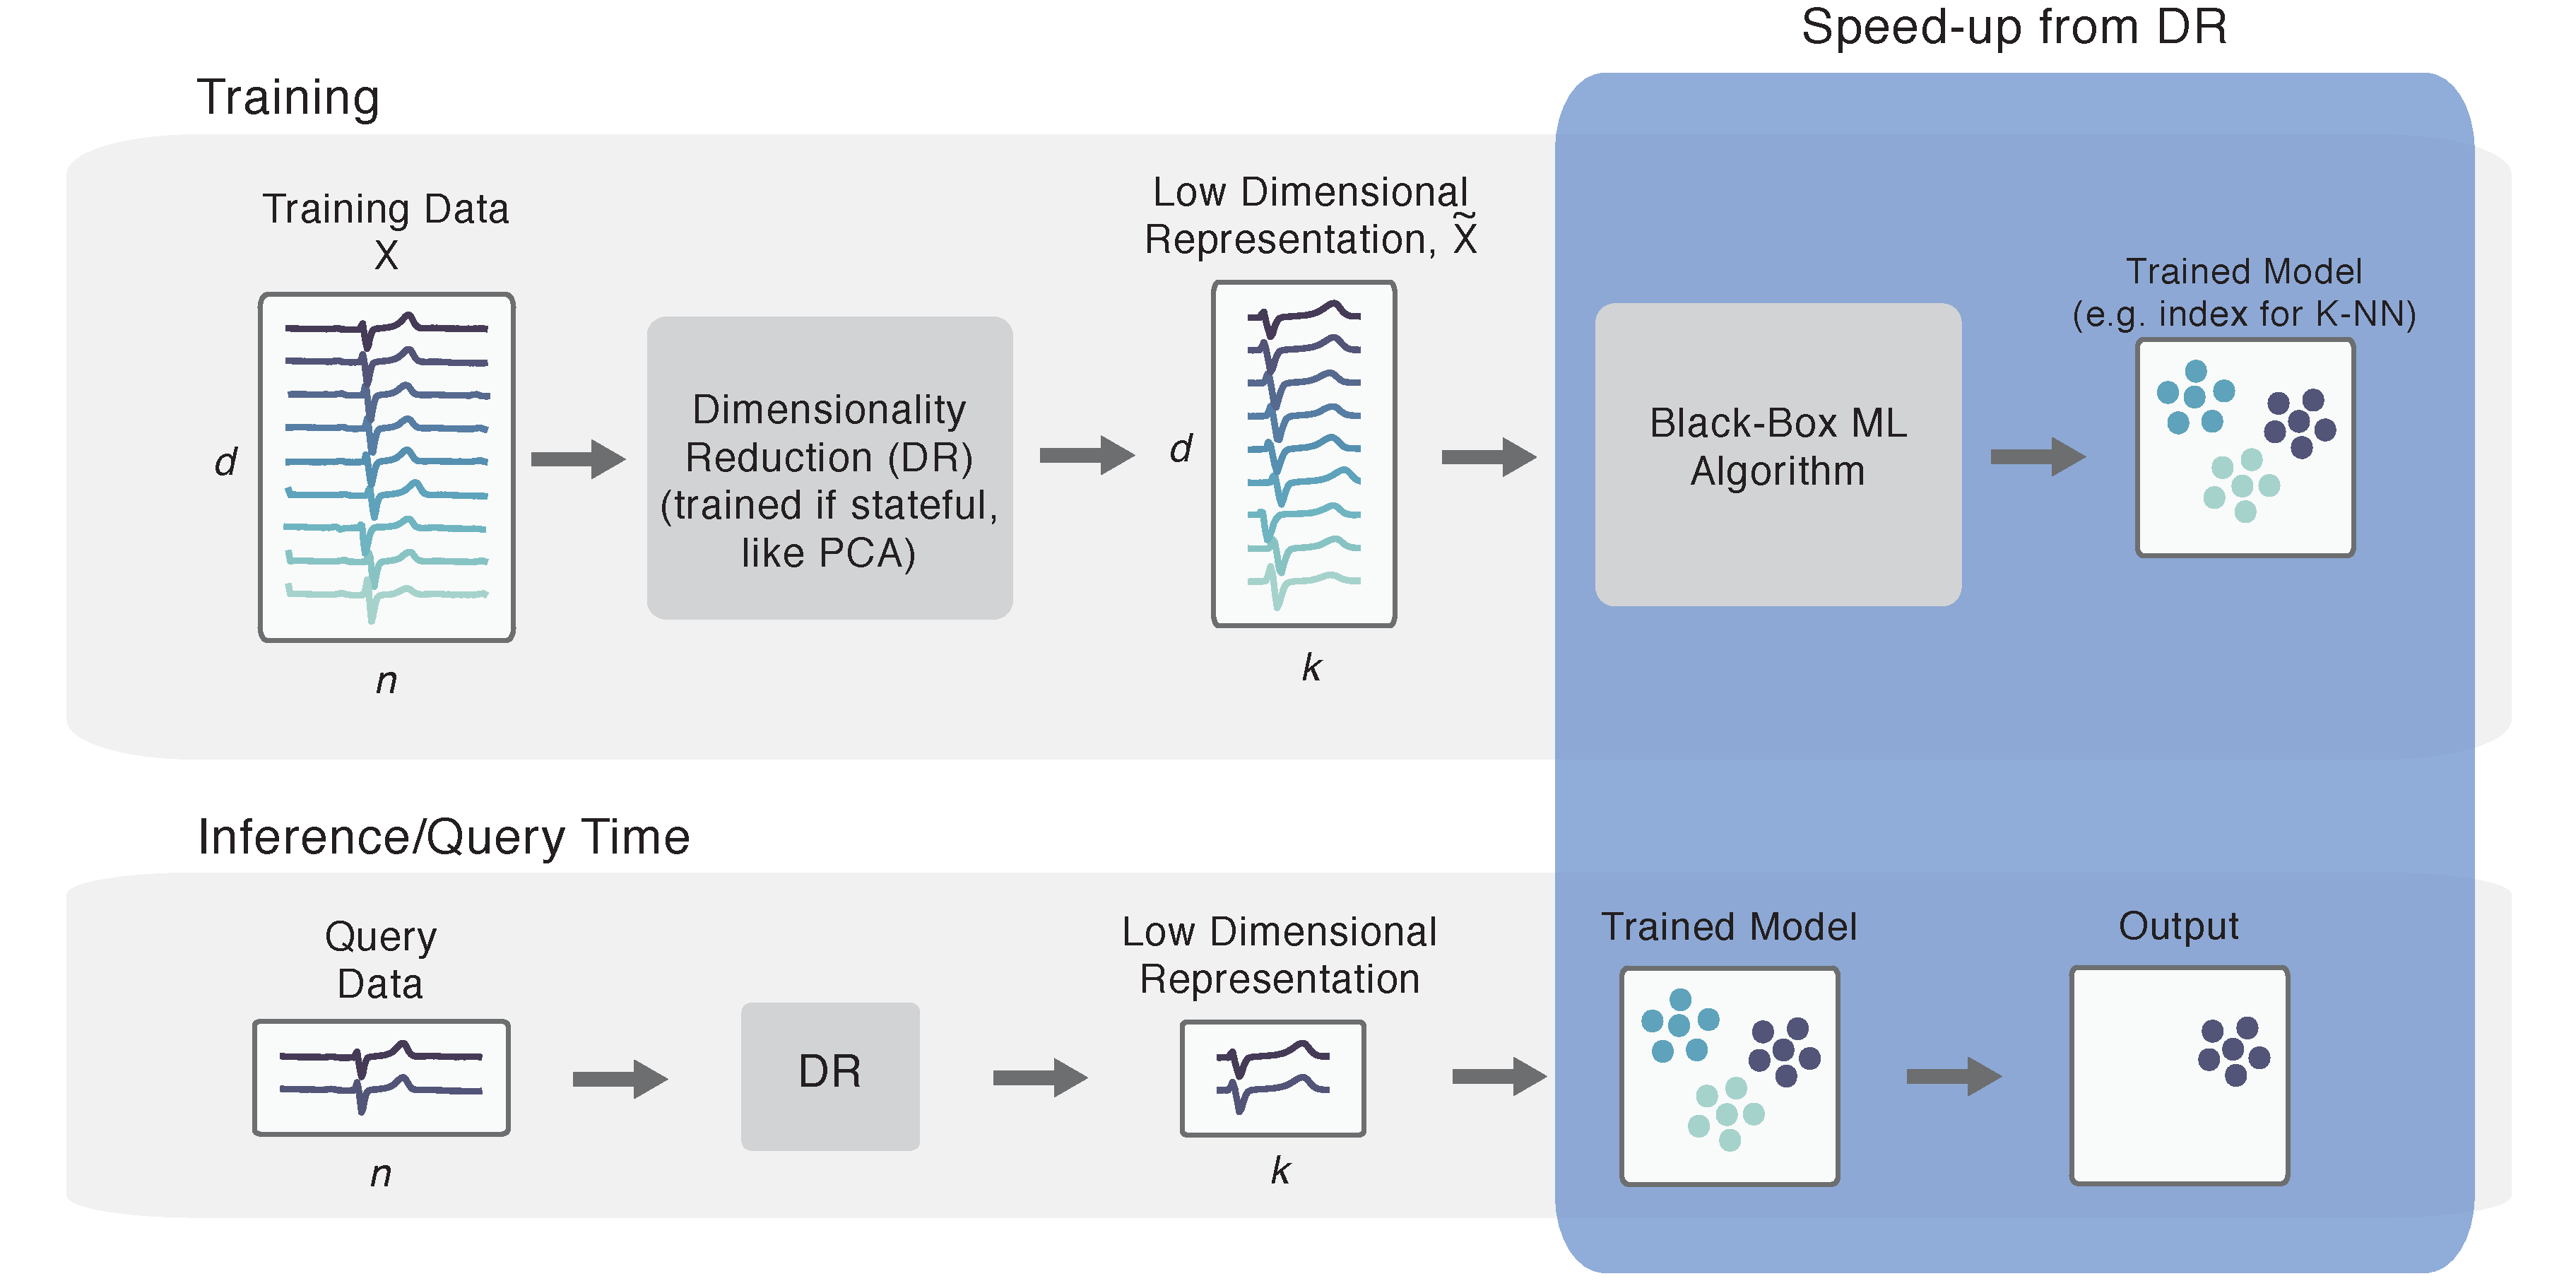
\includegraphics[width=\linewidth]{figs/pipeline.pdf}
\caption[]{Sample machine learning pipeline with dimensionality reduction. Spending time on DR provides downstream runtime speed-ups.}
\label{fig:pipeline}
\end{figure}
\end{comment}

To this end, we develop DROP\footnote{\href{https://github.com/stanford-futuredata/DROP}{https://github.com/stanford-futuredata/DROP}}, a system that dynamically identifies the amount of sampling required for stochastic PCA by using downstream task information.
DROP takes as input a high-dimensional dataset,
%\footnote{Our focus \red{is on time series similarity search,} given the amount of study in the database community~\cite{keogh-study} and resurging interest in time series analytics systems~\cite{macrobase,macrobase-cidr,trill-signal}. 
%We provide preliminary generalizability analyses in \S\ref{sec:experiments}.}  
a property to preserve (e.g., pairwise Euclidean distance to 5\%), and an optional runtime model expressing downstream computational cost as a function of dimensionality (e.g., for k-Nearest Neighbors [k-NN], runtime is linear in dimensionality). 
DROP returns a low-dimensional transformation for the input using as few samples as needed to minimize the projected overall workload runtime while satisfying quality constraints.


DROP addresses the question of how much to sample the input dataset via data-dependent progressive sampling and online progress estimation at runtime.  
DROP performs PCA on a small sample to obtain a candidate transformation, then increases the number of samples until termination (see Figure~\ref{fig:basic}). 
To identify the termination point that minimizes runtime, DROP must overcome three challenges:

First, given the results of PCA on a data sample, DROP must \emph{evaluate the quality} of the current candidate transformation.
Popular analytics and data mining tasks often require approximate preservation of metrics such as average pairwise distances between data points~\cite{time-series-dm,dm-book}, which are costly to compute.
Thus, DROP adapts confidence intervals for fast estimation of the input metric to preserve.


Second, DROP must \emph{estimate the marginal benefit of sampling additional datapoints}.
When running PCA on a series of larger samples, later samples will increase $R$, but may return lower $k$ (lower downstream runtime). 
To navigate this trade-off between end-to-end runtime and transformation quality, DROP uses the results obtained from previous iterations to build a  performance model for future iterations.


Finally, given the expected marginal benefit of the next iteration, DROP must \emph{optimize end-to-end runtime}.
While an application-agnostic approach would iterate until successive iterations yield no quality benefit, a user-provided cost model may reveal that trading a higher $k$ for a lower $R$ may decrease end-to-end runtime.
DROP therefore evaluates this cost at each iteration
to minimize the expected workload runtime.


\begin{comment}

PCA is guaranteed to find the optimal linear transformation with respect to $\mathcal{L}_2$ reconstruction error, popular analytics and data mining tasks (e.g., k-NN~\cite{time-series-dm}, k-means~\cite{dm-book},  kernel density estimation~\cite{wand}) instead require approximate preservation of metrics such as average pairwise distances between data points.
To overcome this challenge, DROP adapts confidence intervals (either via closed-form or, if unavailable, via bootstrapping) for fast estimation of the input metric to preserve.


Since PCA is guaranteed to find the optimal linear transformation with respect to $\mathcal{L}_2$ reconstruction error, we could consider estimating the transformation quality using this quantity.
However, many popular analytics and data mining tasks (e.g., k-NN~\cite{time-series-dm}, k-Means~\cite{dm-book},  Kernel Density Estimation~\cite{wand}) do not use reconstruction error, and instead require approximate preservation of metrics such as average pairwise distances between data points.
A transformation that minimizes reconstruction error is not guaranteed to preserve the pairwise distance by the same amount.
Moreover, na\"ively computing pairwise distances as required for k-NN is prohibitively expensive, with quadratic runtime.
To overcome this challenge, the system adapts an approach pioneered for deterministic queries in the context of online aggregation: treat quality metrics as aggregation functions and use confidence intervals (either via closed-form or, if unavailable, via bootstrapping) for fast estimation.
This approach allows DROP to accurately estimate representation quality while avoiding the overhead of exact computation.

Second, DROP must \emph{estimate the marginal benefit of continuing to sample} for another iteration.
When running PCA on a series of progressively larger samples, later samples will incur higher computational cost but may in turn return lower-dimensional transformations. 
To navigate this trade-off between end-to-end runtime and transformation quality, the system performs online progress estimation, using the results obtained from previous iterations to build a predictive performance model for future iterations.
%This allows DROP to quantify the expected benefit of continued sampling.

Finally, given the current quality and expected marginal benefit of the next iteration, DROP must \emph{optimize end-to-end runtime} to determine whether to terminate.  
The system must evaluate if the expected marginal benefit to dimensionality arising from continuing to iterate would reduce total runtime.
While an application-agnostic approach would iterate until successive iterations yield no benefit to quality, many analytics operators such as k-Nearest Neighbors are tolerant of error~\cite{gemini}, so it is frequently advantageous to trade a slightly higher-dimensional basis for faster pre-processing (DR).
To address this challenge, the system performs workload-specific optimization to minimize the expected runtime of the complete end-to-end analytics pipeline.
\end{comment}

\begin{comment}
A simple, application-agnostic approach to addressing this problem would iterate until until successive iterations yield no benefit to quality, thus converging to the lowest-dimensional metric-preserving transformation.
However, as we have hinted, many time-series analytics operators such as k-Nearest Neighbors are tolerant of approximation error~\cite{gemini}, and it is frequently advantageous to trade a slightly higher-dimensional basis for faster pre-processing. In these settings, running to convergence is often wasteful.
To address this challenge, DROP performs a workload-specific optimization, utilizing a provided (or profiled) application-specific runtime model and performs online optimization  to minimize the expected runtime of the complete end-to-end analytics pipeline.
\end{comment} 

DROP is a system that combines recent theoretical advances in DR and classic techniques from approximate query processing for end-to-end workflow optimization.
In this work, we make the following contributions:
\begin{itemize}

\item We show the data sample required to perform accuracy-achieving PCA is often small (as little as $1\%$), and sampling can enable up to \red{$91\times$} speedup over baseline PCA. 
%We show that as little as $2\%$ of time series data suffices to preserve pairwise distances within $2\%$, providing a $55.6\times$ reduction in dimension.
  %this came from the oracle numbers--used 0.002 and then looked at table
  
\item We propose DROP, an online optimizer for DR that uses information about downstream analytics tasks to perform efficient stochastic PCA.
%. DROP uses information about downstream analytics tasks to utilize as few samples as required to minimize the overall workload runtime, while satisfying constraints on the reduction quality.

\item We present techniques based on progressive sampling, approximate query processing, online progress estimation, and cost based optimization to enable up to \red{$5\times$} faster end-to-end execution over PCA via SVD.% and up to $3\times$ faster end-to-end execution than alternative techniques on real analytics pipelines.
\end{itemize}



